\newpage
\section{Executive Summary}

\tess is scheduled to launch in December of 2017.
The primary mission will run for two years, and the \tess Science Office will submit a proposal for an extended mission to NASA's senior review of operating missions in early 2020.
In this report we lay out technical requirements, science goals, opportunities, and risks that will impact the decision of how \tess should observe after completing its primary mission.

\begin{figure*}[!b]
	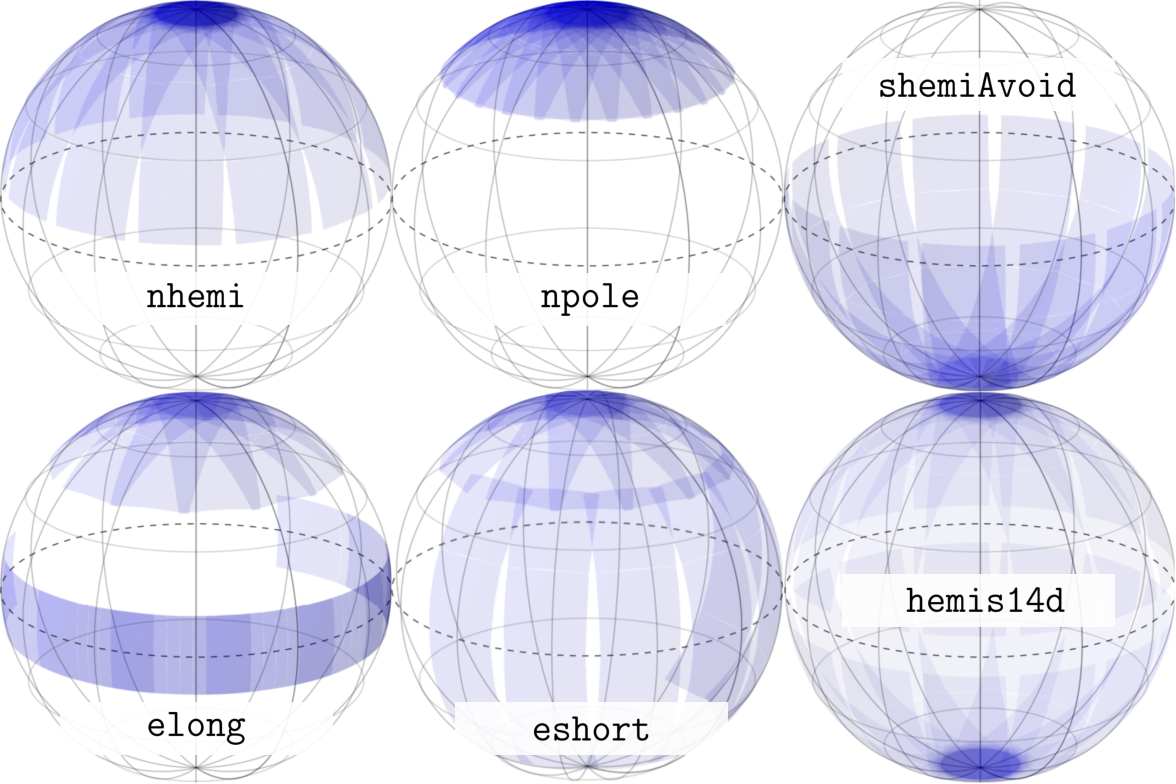
\includegraphics{figures/proposed_pointings_texttt.pdf}
	\caption{Six proposed pointing strategies for a \tess extended mission, visualized in ecliptic coordinates.
	Earth and moon crossings make looking at the ecliptic for an entire year impractical (see Fig.~\protect\ref{fig:earth_moon_elong}).}
	\label{fig:strategies}
\end{figure*}
%!WINN!: begin with broader discussion
%!BOUMA!: about what?
Building on \citet{Sullivan_2015}, we perform Monte Carlo simulations of the population of planets that \tess will detect for the Year-3 observing strategies shown in Fig.~\ref{fig:strategies}.
None of our proposed strategies entail observing the ecliptic for an entire year.
For $\sim\!4$ months of such a scenario, the Earth and Moon cross \tesss field of view at a drastically higher rate than during the rest of the year (Fig.~\ref{fig:earth_moon_elong}).
We circumvent this issue by proposing \elong\ and \eshort.
We also note in passing that \hemis\ spends a single spacecraft orbit ($\sim$14 days) per field, `zig-zagging' across the sky.


The most notable result from these simulations is that a third year's extended mission will yield as many new sub-Neptune radius planets as either Years 1 or 2 -- roughly $1250$.
The means that extended missions will be valuable because they will detect a large number of small planets.
This holds regardless of where on the sky observe, with the newly detected planet yields varying by $\lesssim 30\%$ between our six proposed scenarios.

Another notable result is that it will be possible to detect about as many new $P>20$ day planets in one year of \tesss extended mission are in both years of the primary mission.
This result derives both from turning high-SNR single-transit events from the primary into double and triple-transit events (giving more transits over which to phase-fold and lower the in-transit noise), as well as by turning low-SNR multiple-transit events into threshold-crossing\footnote{Following \citet{Sullivan_2015}, we rule a planet detected if $\mathrm{SNR} > 7.3$ and $N_\mathrm{tra}\geq 2$.} events.

An additional result, relevant to both the primary and extended missions, is that our simulations approximate the effect of the Earth and Moon crossing through \tesss field of view (Sec.~\ref{sec:earth_moon_crossings}).
Running the primary mission without accounting for Earth and Moon losses returns a mean of 2678 detected planets with $R_p<4R_\oplus$, while running them with Earth and Moon crossings gives 2482 such planets on average.
This is a loss of 196 planets, or $7\%$ of the sub-Neptune yield.


\paragraph{Assessing pointing strategies based on yield statistics} 
Different extended mission pointings perform better and worse by different metrics.
We focus only on detected planets with $R_p<4R_\oplus$ (Fig.~\ref{fig:yield_results}).
In terms of absolute sub-Neptune radius planet yield, \hemis, \npole, and \shemiAvoid\ offer the most new planets (1300-1400, compared to the primary mission's 2500).
\hemis, \npole, and \nhemi\ offer the most new long period planets (250-300, compared to the primary mission's 290).
\hemis, \shemiAvoid, and \eshort\ offer the most new planets orbiting $I_c<10$ hosts ($\sim$190, compared to the primary's 385; see Table~\ref{tab:icmag_meta}).
%cf bright_star_comparison_Ic_lt_10.ipynb
They all offer similar numbers of new habitable zone planets (about 120, to the primary's 210)\footnote{We let `habitable zone' mean that the planet insolation $S$ is within $0.2S_\oplus-2S_\oplus$. The physically-motivated~\protect\citet{kopparapu_habitable_2013} HZ gives roughly a third of our quoted numbers (Fig.~\protect\ref{fig:scatter_habitable_zone}).}.
\npole\ is the worst at detecting new planets with atmospheres that are amenable for atmospheric follow-up, but extended missions only yield $10-25$ such planets, compared to the primary mission's $\sim$110.\footnote{We let `amenable for atmospheric follow-up' mean $\mathrm{SNR}_\mathrm{atm} > \mathrm{SNR}_\mathrm{GJ\ 1214b}/4 $, where $\mathrm{SNR}_\mathrm{atm}$ refers to the signal-to-noise of the planet in transmission over 4 transits observed by \jwsts NIRISS instrument, and the normalization is $\mathrm{SNR}_\mathrm{atm}$ for GJ 1214b. Dividing by a factor of four helps avoid small-number fluctuations. Note for \textit{JWST} follow-up the ecliptic latitude of the detections also matters (see following footnote).}
%!WINN! explain why, in brief
%!BOUMA! at what level of detail? "this is why, order of magnitude, for all?" I'm not sure what explanation is needed except that strategies are optimizing for different criteria... between total sky area, amount of overlap between sectors, ...

An important assumption behind these statistics is that we assume 2 transits and a phase-folded SNR of 7.3 are sufficient for detection.
\hemis\ is more dependent on this assumption than any other scenario: it detects the most new planets and the most new $P>20$ day planets, but if we were to modify our detection requirement to $N_\mathrm{tra}\geq 3$, roughly half of the long period planets that \hemis\ detects would be lost (Fig.~\ref{fig:Ntra_hist}).
Given the overwhelming amount of false alarms that will be present in a transit-search pipeline from $N_\mathrm{tra} = 2$ events, this is a serious caution against the \hemis\ approach.
By way of comparison, \npole\ detects most of its long-period planets with $\ge 4$ transits.


\paragraph{Desires in exoplanet science:}
Planet yield statistics are useful, but they are blind to other important considerations. For an extensive discussion of the broad science that can be accomplished with extra \tess observations, see LINK!; for a discussion of which opportunities we think affect extended mission planning, see LINK!. Summarizing,

\textit{1.) Ephemeris times:}
The \tess mission must provide accurate predictions for when its objects transit to enable successful follow-up efforts.

Following a derivation shown in Sec.~\ref{sec:ephemeris_times},
the uncertainty on the mid-transit times for \tess objects of interest, $\sigma_{t_c}$, propagates to be roughly
$$\sigma_{t_c}\ \mathrm{[hr]} \approx 2\times\left(\mathrm{number\ of\ years\ after\ detection}\right). $$
This problem is reduced by an order of magnitude if we capture just one transit with a year's baseline after the initial detection (Figs.~\ref{fig:lowering_uncertainty_tc},~\ref{fig:conf_interval_gets_better}).
This argues strongly for an extended mission which, whether over 1 or 2 years, re-observes many of the targets that \tess detects in its primary mission. 
The smallest-radius Earths and super-Earths may otherwise be difficult to recover.

\textit{2.) Follow-up of \tess objects}\newline
\textit{2.1) JWST:} \tess should detect the most promising planets for \jwst follow-up\footnote{We let `promising planets for \jwst follow-up' mean those that have $R_p<4R_\oplus$, $\mathrm{SNR_{atm}} > \mathrm{SNR_{GJ\ 1214b}}/5$, and absolute ecliptic latitude $|\beta|>80^\circ$ so that they can be observed for more than two-thirds of the year by \jwst\!.} after only a year's observation (see table \& discussion at LINK!).
This means that \tess is not `bound' to the ecliptic poles in an extended mission to support \jwsts target selection.
More important for ensuring \jwst\!--\tess overlap will be the efficient spectroscopic and photometric follow-up of \tesss planets from the ground; by \jwsts launch in October 2018, only a few verified \tess planets will be known.

\textit{2.2) CHEOPSs'} visibility is best near the ecliptic, and non-existent near the ecliptic poles.
Extended missions that focus exclusively on the ecliptic poles neglect \tess and \cheopss complementarity~\citep{berta_cheops_2016}.
Those that focus on the ecliptic, including \elong\ and \eshort, provide the largest amount of overlapping coverage, with \nhemi\ providing a middle-ground.

\textit{2.3)} 
The primary mission will clarify whether the availability of \textit{ground-based follow-up resources} will need to constrain \tesss extended observing.
Ideally, it will not.
%!WINN! ?
%!BOUMA! for instance if there were more telescopes in the north, TESS should maybe observe in the north to make sure its planets get followed up.

\textit{3.) \tess as a follow-up mission:}
\tesss target list in the primary mission will include known planet-hosts from transit and RV surveys.
Summarizing those that are most strategically important for an extended mission:

\textit{3.1) The Kepler field.} \tess observes the \kepler field for $\sim$52 days in 2019 (Fig.~\ref{fig:positions_pointings}).
An extended mission like \npole\ could observe the field for 104 days per year -- twice as long as repeating \nhemi.
The main reasons to allocate extra importance to \keplers field include:
\textit{(a)} measuring transit timing variations over a long baseline;
\textit{(b)} confirming few-transit KOI candidates, 
\textit{(c)} calibrating \tess against well-studied candidates,
\textit{(d)} continuing observations of circumbinary planets.
\citet{sullivan_KOIs_2013} studied \tesss performance on the field in detail.
Scaling his absolute results by a factor of $1.5$ (about twice as many KOIs are now known, but they are systematically fainter), we can expect \tess to detect $\sim$45 $R_p<4R_\oplus$ KOIs at $\geq3\sigma$ per transit.

\textit{3.2) K2's fields} will have covered $\gtrsim\!60\%$ of the area in the $|\beta|<6^\circ$ band about the ecliptic by the beginning of \tesss extended mission %\footnote{18 campaigns, with a 115 square degree field of view. 17 fields do not overlap (much).}.
\tesss primary mission does not observe in the $|\beta|<6^\circ$ band. 
Our simulated planet populations for both \elong\ and \eshort\ assumed no knowledge from \ktwo\!.
This is unrealistic.
A large fraction of the planets that \tess will be capable of detecting near the ecliptic will already either exist as candidates in \ktwos data or have been discovered\footnote{Our coarse estimate is that $\sim$175 of \tesss 500 new $|\beta<12^\circ|$, $R_p<4R_\oplus$ detections from \elong\ would already be detected by \ktwo (see Sec.~\protect\ref{sec:risks_opps})}.
%For a scenario like \elong, the average \tess coverage per star over the extended mission in the $\pm12^\circ$ band would be $\sim$7 spacecraft orbits, or $\sim$91 days of near-continuous observing (to \ktwos $\sim$80).	
Summarizing then what we find to be the most compelling reasons to observe the ecliptic in an extended \tess mission:
\textit{(a)} combine \tess and \ktwo data, doubling the \ktwo observing baseline for most targets. In turn, confirm low-SNR candidates, and detect extra transits for a relatively large number of $20<P<40$ day planets;
\textit{(b)} catch `holes' in the $|\beta| < 12^\circ$ band that \ktwo missed, completing the all-sky search for small planets transiting the brightest stars;
\textit{(c)} observe targets in \ktwo fields that simply were not selected in \ktwos $\sim\!2\times10^4$ per campaign. For instance, \tesss bandpass allows probing down to cooler M dwarfs;
\textit{(d)} measure TTVs for targets over baselines up to 5-years.
\textit{(e)} confirm a small but significant number of $P>40$ day planets.

Given the central role that combining \tess and \ktwo data would play if \tess were to observe the ecliptic, and given our non-treatment of this question in our yield simulations, we recommend that a detailed study of \ktwo and \tesss combined potential be carried out before ruling for or against \elong\ or \eshort.

\textit{3.3) \tess following up ground-based surveys:}
%\tesss photometric precision provides the greatest relative benefit for planets that have never been observed from space.
The north and south skies have similar numbers of known ground-detected transiting and RV planets, so the desire to follow up ground-based surveys probably will not impact \tesss extended mission on a 1-year timescale.
Over 2-year timescales, if an extended mission were to focus on a single hemisphere it would neglect half of the known transiting/RV planets, no longer \textit{(a)} discovering additional small transiting companions %(\`a la WASP 47) 
or \textit{(b)} improving uncertainties in the physical and orbital parameters of known planets.


\paragraph{Desires outside of exoplanet science:}
We motivate cases for using \tess data in asteroseismology, variable-star astronomy (pulsating stars, eruptive stars, supernovae), and solar system astronomy (main belt asteroids) at LINK!.
To our understanding an extended mission can observe anywhere on the sky without neglecting these sub-fields.
%!WINN! ? (about the above sentence)
%!BOUMA! I'm trying to tie all of this to extended missions. If any of the broader science restricts where we can observe in an extended mission, this is where I would say it. I don't think it does though. Hence the above sentence.
Observational cadence is a more important free-parameter -- asteroseismology in particular benefits greatly from short cadence data.


\paragraph{Results summary:}
\begin{description}
	\item[1 year extension:]
%	If you don't waste months looking at the Earth and Moon, you can look anywhere and find many planets. 
	None of the pointing options that we propose are obviously bad (Fig.~\ref{fig:yield_results}).
	\hemis\ does well under idealized assumptions, but is risky because of aliasing and low $N_\mathrm{tra}$ issues. 
	However it could be the fastest way to deal with the ephemeris issue.
	The biggest qualitative difference between looking at and away from the ecliptic is \textit{K2}.
%	I ignored this issue.
	\textit{K2} does mean fewer `new \tess planets', but combining the two datasets might lead to many long period planet detections (see recommendations -- we did not deal with this quantitatively).
	
	\item[2 year extension:]
	Knowing when \tess planets transit is incredibly important for follow-up efforts, and needs to be addressed either through \hemis\ or by going `all-sky' over two years.
	Although we did not study 2-year extensions in depth, performing the opposite-hemisphere complements of \nhemi, \npole, and \shemiAvoid\ would yield the same large number of new planets as from Year 3.
	Another reason to observe both hemispheres is to be sure that we have really detected all of the best super-Earths for transmission spectroscopy (Table~\ref{tab:jwst2}).
	
	The main reason to repeat one-hemisphere observations indefinitely is to detect long period planets.
	Our opinion is that the reasons to observe all-sky are more compelling.
	
\end{description}



\paragraph{Recommendations (expanded in Sec.~\ref{sec:recommendations}):}

\begin{description}
	\item[Analyze target prioritization problem:] planet occurrence rates are functionally dependent on a star's properties -- should this affect which stars we give upgraded cadence?
	Is our proposed \texttt{Merit} statistic (Eq.~\ref{eq:merit}) how we want to prioritize target stars for short-cadence observations?
	%for instance \'a la~\protect\citet{kipping_transit_2016}. 
	
	\item[Optimize cadence:] it may be better for transit detection to observe $4\times10^5$ target stars at 4 minute cadence, rather than $2\times10^5$ at 2 minute cadence.
	
	\item[Take steps to address the `upgrading cadence' problem:] 
	if there is a likely transiting planet in full frame image data, upgrading the planet to short cadence in future observing sectors improves the probability and quality of detection.
	
	\item[Guest Investigator Office / \tess Science Office: solicit advice]
	from experts in asteroseismology and variable-sky astronomy to understand how extended missions affect their science cases (\textit{e.g.}, data throughput rates are particularly important for time-sensitive supernovae observations).
	More broadly, solicit community feedback during the process of defining the extended mission.
	This may entail a call for white papers, comments on this report, or direct proposals to the GI office. 
	%As exemplified in NASA’s 2016 Astrophysics Senior Review, everyone benefits from the discussions generated by such community feedback~\citep{donahue_senior_2016}.
	
	\item[Decide (explicitly or implicitly) on weights between our proposed metrics.]
	Sec.~\ref{sec:comparing_pointing_strategies} gives a list of considerations that will matter in deciding \tesss extended mission: should we prioritize new planet detection statistics? Broader astronomy, as \ktwo did?
	Are the $\lesssim30\%$ variations in absolute new planet yields more valuable than other desires or opportunities?
	
	\item[Simulate combining \tess and \ktwo data for \rm{\elong\ } \textit{and} \rm{\eshort}.] 
	This is perhaps the most important qualitative difference between observing towards and away from the ecliptic.
	%Would \tess\!+\ktwo enable more discoveries out at long periods than alternatives?
	%How many of the new planets that \tess detects on the ecliptic will actually be detected by \ktwo?
	%Is the value-added of combining datasets a compelling case compared with discovery?
	
	%\item[Further topics for study:]
	%\textit{1.)}
	%Would observing \npole\ for 2 years hit the `low-hanging fruit' barrier?
	%How much dimmer would the host stars of new planets be in such a scenario?
	%Would the planets tend to be smaller?
	%Would there be fewer of them?
	%\textit{2.)}
	%Study the limiting case of \hemis\ for 2 years, vs primary mission repeat for 2 years, vs \npole$\times$2 for 2 years. The most interesting aspect here is the continuous viewing zones: 2 CVZs at 14-day sampling, vs. 2 CVZs at continuous sampling for one-year each, vs. 1 CVZ for full sampling over two years.\footnote{Our simplified perfect period extraction would miss challenges from the data processing.}
\end{description}

\newpage













\begin{comment}
\textit{Targets beyond cool bright dwarfs:} there are many classes of targets we may wish to observe with \tess, possibly for exoplanet science, and possibly for other astronomy/astrophysics (\textbf{see K2 page for list. Solar system, extragalactic, exoplanets, ...}).

In exoplanets, following up on the \kepler field promises a substantial scientific return, though mainly for science beyond planet discovery (measuring transit timing variations, refining ephemerides, building SNR on few-transit candidates).
There are numerous non-\kepler transiting planets that should be considered: these will be observed during the primary mission, and will have a relatively larger `value-added' than the KOIs in terms of improved photometric precision and detection of smaller companions.
On the ecliptic, observing the \ktwo field would let us do \textit{this, that and the other}, but would mean losing long-term coverage at an ecliptic pole, a noiser field (Earth/Moon crossings, zodicial background, main-belt asteroids).

Other subfields of astronomy would argue it in different ways. 
Asteroseismic targets are wherever we look.
There are no known open clusters near the North Ecliptic Pole, and there are a handful near the South.
Variable stars will be everywhere, but the best-characterized fields are the MACHO and OGLE-III/IV fields near the South Ecliptic Pole.

\paragraph{Risks and opportunities in exoplanet science}


\textbf{Earth and Moon crossings}
This work took a na\"ive approach towards modeling the Earth and Moon crossing through \tesss field of view: informed by detailed calculations of how common these crossings will be, we simply \textit{dropped} a corresponding number of fields from our planet yield calculation.
This lowered the yield of $R_p<4R_\oplus$ planets by $\sim\!10\%$.
Given that Earth/Moon crossings typically last for a small fraction of an orbit (Fig.~\ref{fig:earth_moon_primary}), if the timescales required for the cameras to `re-settle' after the crossings are small compared to orbital timescales, then our approach over-estimates the effect.

\textbf{What's best for two years of extended observing?}
The fact that \tess can detect many small planets orbiting bright stars across the sky strong argues towards continuing observing `all-sky', rather than focusing observations on a single ecliptic hemisphere after the primary mission's completion.

Reasons to do all-sky two years: ephemerides for \tess planets; detect just as many new planets as from Year 3; 
Reasons to do one-hemisphere for eternity: long period planets

that none of our extended mission pointing scenarios produce yields that are that different:
for a single year's extended mission, \textbf{none of the extended missions proposed here are exceptional stand-outs}.
In terms of raw planet detection statistics (what gives the most new planets? at the longest periods? \&c.) \hemis, \npole, 

An important follow-up: \textbf{but they are slightly different}.
\end{comment}
